\section{Preliminary Results}

In this section, we evaluate the performance of the state-of-the-art robust
SLAM method, the Max-Mixture algorithm, given dynamic landmark measurements.
Max-Mixture is a robust extension to classical graph SLAM using Gaussian
mixture in factor representation, that is, $ x_i = \sum_c \phi_c
\mathcal{N}(\mu_c, \Sigma_c)$ for component $c$ and weight $\phi_c$, with
obvervations being components, also similarly for $z_i$. Max-Mixture uses a max
function to approximate and efficiently evaluate the sum of Gaussians. It is
well-known for its capability of handling a large amount of incorrect loop
closures, but it is untested against moving landmarks, and this experiment can
be representative to other approaches in the robust SLAM literature. 

We apply different perturbations to a single landmark (landmark 249) in the
Victoria Park dataset, and compare the different effects of the perturbations
on the optimal estimate of the trajectory and the map of all landmarks obtained
by Max-Mixture graph SLAM. The Victoria Park dataset contains 2-D odometry and
landmark observations. As shown in figure \ref{fig:baseline} the left plot is
the control group without perturbation, and is accurate to the ground truth. A
single southward bias is applied to all observations of the
landmark in the middle plot, simulating sensory outliers. A temporally
increasing bias is applied to all observations of the landmark in the right
plot, simulating a southward moving landmark.

\begin{figure}[h]
\makebox[\textwidth][c]{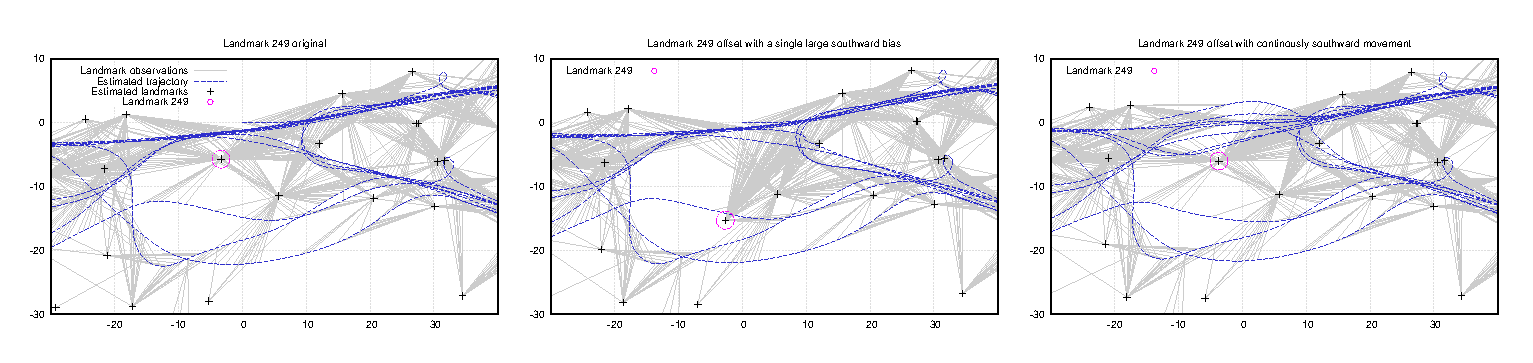
\includegraphics[width=\textwidth]{fig/baseline-mm}}
\caption{The optimal estimates of the trajectory and landmark positions
obtained by Max-Mixture graph SLAM.  Left: low convergence uncertainty. Middle:
high convergence uncertainty because of rejection of outlier observations
of landmark 249.  Right: low convergence uncertainty, no outlier
detected by Max-Mixture.}
\label{fig:baseline}
\end{figure}

As the middle plot shows, Max-Mixture is still capable of handling noise of
large bias or spurious loop closures introduced by simluated sensory fault. It
correctly rejects outlier landmark observations and recovers the position of
the perturbed landmark. However, it completely fails to reject any unlikely
landmark observations and largely distorts the resulting trajectory when given
moving landmark measurements. An explanation for this is that each clique of
landmarks with coherent motion forms a plausible reference frame for related
observations. Inference based on each independent reference frame will reach
plausible estimate of robot trjectory and the map, however robust SLAM methods
which assume stationary landmarks will average over a sum of different
reference frames and lead to wrong conclusions.

%%%%%
To benchmark the robustness of the proposed approach and to show its correctness and feasibility, we used the Victoria Park dataset that has been used in a number of publications before. The dataset consists of pose graphs in 2D and contain several thousand poses and landmark constraints. We corrupted the data by setting landmark ``249" (circled in red) in a constant northward movement, where its eventual position is roughly 7 meters north of its original location. We chose landmark ``249" due to the relatively large amount of observations on this particular landmark in the dataset. We expect the more observations there are on a landmark, the greater its movement would corrupt the final optimization results and the more possible that existing robust SLAM methods would fail. \\

%% TODO: Some explanations about DCS and SLAM w/ EM

%% TODO: Add figures
\textbf{TODO:} figures (7-meter movement, 14-meter movement, from the presentation) \\


[Fig. ...] shows the results for DCS, simple EM, and our approach. As expected, current state of the art frameworks are not able to cope with the outlier constraints and converge towards defective solutions. This is particularly illustrated in the lower left figure of [Fig. ...], which shows the results of simple EM algorithm with weights only added to the landmarks. Even g2o with robust DCS cost kernel is not able to converge correctly, where we can see pose graph around the moving landmark is clearly distorted. Our robust back-end however, is able to converge to a correct solution in a few iterations. The outlier is correctly deactivated by driving their associated weights $w_{j_k}$ and $v_k$ close to zeros. 



%% TODO: figures showing the learning objective 
\textbf{TODO:} ``To help verify that your statistical learning algorithm is working properly, at least one plot showing the learning objective (joint log-probability for an MCMC method, a log-likelihood bound for a variational method, etc.) as a function of the number of learning iterations."  

(Final or initial $\chi^2$ errors against number of iterations)  \\




